\documentclass{IEEEtran}

\usepackage{mathtools}
\usepackage{graphicx}
\usepackage{subfig}
\usepackage{verbatim}
\usepackage{algpseudocode}
\usepackage{natbib}
\usepackage{url}

\begin{document}

\title{Paper Currency Recognition with Color Histograms}
\date {November of 2012}
%\author{Sebastian Gomez \\ Tatiana Lopez}
\author{\IEEEauthorblockN{Sebastian Gomez, Tatiana Lopez Guevara \\}
\IEEEauthorblockA{School of Computer Engineering\\
Universidad Tecnologica de Pereira\\
Pereira, Colombia\\
Email: sebasutp@gmail.com, tatiana.lopez@sirius.utp.edu.co }}
\maketitle


\begin{abstract}
This document shows an approach to make a color histogram based classification of paper currency from an image.
First, it exposes how the features were extracted from the images and how to classify them once those features
are extracted. Finally, it explains how the results were obtained and shows the analysis of the results.
%todo:Terminar abstract
\end{abstract}

\begin{IEEEkeywords}
Artificial neural networks, classification algorithms, machine learning.
\end{IEEEkeywords}

\section{Introduction}
\IEEEPARstart{F}{or} blind people in many countries it is hard to recognize the denomination of their local paper currency because
there are not enough non optical features in the bills. It would be useful for them to have an automated software that
can recognize the currency denomination from an image.

%There are several publications on these kinds of systems. %todo: Mention them

Our approach uses only color information, but the accuracy might be improved by adding features that make use of
texture information. This document explains the methodology used to extract the features, to make the classification
of the paper currency and to analyze the results. The goal is to classify the Colombian paper currencies based only
on color features, the denominations of the Colombian currency are \$1000, \$2000, \$5000, \$10000, \$20000 and
\$50000.

\section{Methodology}

The classification system consist of a feature extraction part, whose responsibility is to compute a vector of
fixed dimensionality. That feature vector is then given to a machine learning algorithm to classify the input
into one of the corresponding classes.

\subsection{Feature extraction}

The features used in this system are only color based features. RGB is a color model that expresses the color of
each pixel as a vector in a 3-Dimensional space, whose components represent the intensities of red, green and blue
channels respectively. This model is widely used for screens, cameras and other optical devices but its disadvantage is 
that it mixes color and brightness information. As the idea is to classify bills regardless of the how bright or 
dark is the scene, some degree of brightness invariance in the feature vector is desirable.

In order to achieve invariance to brightness in the images, a color model created by cielab was used %cite
named Yxy, where the Y channel carries the brightness information while x and y are the chrominance (color) 
channels. To transform RGB to Yxy and viceversa a linear transformation, followed by a normalization are
performed. Brightness invariance is obtained when each pixel in the image is transformed to Yxy and the
Y channel is dropped, this color model is called xy and from it you can not obtain the original image.

One very used technique to extract color information is to generate color histograms. For each pixel
the bin were it falls must be determined, and the final output is the count of how many pixels fall
into each bin. As the color information used is 2-Dimensional (xy model), the amount of histogram
bins grow quadratically with the number of division used for each dimension. 

For example, suppose that both x and y vary from 0 to 100. And that the bins intervals are each 5
units, so you would have 20 division in each dimension. The bins would look like a 20 by 20 matrix
and the goal is to count how many (x,y) points fall into each slot of the matrix (bin). Note that
it that case there would be $20^2=400$ different bins.

The problem with that approach is that, as the points do not distribute uniformly, some bins might
never be used at all while some other could end up having most of the points. Instead of choosing the
bins that way, a K-Means algorithm was run over the input points to choose the bins. By doing so
the centroids would not be placed in regions were there are not any points and hopefully in the
regions were there are more points more centers would be placed. To determine the bin were each pixel
falls the closest centroid to that point must be computed using the euclidean distance.

In summary, the feature vectors used for this work were computed as color histograms in the
xy color model space. And the histogram bins were computed using k-means, where k is the
amount of bins desired for the histogram.

%todo: Append images modifying Yxy brightness

\subsection{Classification system}

\subsubsection{Linear classifier}
The optimization algorithm used to find the weights $\vec{w}$ that minimized the classification error on the training 
set was conjugate gradient.
Since this work is focused in a multiclass classification problem, the functions employed to calculate the output $\vec{y}$, the error $E$
and derivatives of such error with respect to the weights $\nabla E$ were the softmax function (eq. \ref{eq:softmax}), 
the cross-entropy error function (eq. \ref{eq:crossee}), and the error gradient (eq. \ref{eq:gradSoftMax}) respectively.
\begin{align}
E(\vec{w}) &= -\sum_{n=1}^{N}{\sum_{k=1}^{K}{\vec{t}_{n,k} \ln \vec{y}_{k}(\vec{w},\vec{x_{n}})}} \label{eq:crossee} \\
\nabla E(\vec{w}) &=  \sum_{n=1}^{N}{(\vec{y}_{n} - \vec{t}_{n})*\vec{x}_{n}} \label{eq:gradSoftMax}
\end{align}

Where $N$ corresponds to the number of training instances, $\vec{x}$ is the feature vector, $K$ is the number of classes
and $\vec{w}$ is the weight matrix composed of $N$ rows and $K$ columns, giving K discriminant functions one for
each class. The known output of the training set $\vec{t}$ is also a matrix of $N * K$ dimensions, where for each row, 
there is only a value of 1 at a column k, indicating that such training row belongs to class k.

\subsubsection{Multilayer perceptron}
The multilayer perceptrons used in this project used a sigmoid function (eq. \ref{eq:sigmoid}) as the
activation function for the hidden layers and a softmax function (eq. \ref{eq:softmax}) for the output layer
because the task of classification is for multiple classes as explained on \cite{alpaydin2004}.

\begin{align}
\sigma(x) &= \frac{1}{1+e^{-x}} \label{eq:sigmoid} \\ 
S_j(\vec{x}) &= \frac{e^{x_j}}{\sum_{i=1}^D{e^{x_i}}} \label{eq:softmax}
\end{align}

The network was trained using back propagation algorithm to compute the gradients and the complex conjugate
optimization algorithm was used to find the weights that decrease the network error on the training set on
each iteration. Let $W_{hj}$ be the weight of the input value $j$ to the hidden neuron $h$, and $V_{ih}$ be
the weight of the hidden neuron output $h$ to the output neuron $i$. Then the gradients are computed as:

\begin{align}
\Delta V_{ih} &= \sum_{t=1}^{N}{(Y_{ti} - R_{ti}) \hat{Z}_{th}} \label{eq:gradV} \\ 
\Delta W_{hj} &= \sum_{t=1}^{N}{ 
    \left[ Z_{th}(1 - Z_{th})\hat{X}_{tj} \sum_{i=1}^{K}{ (Y_{ti} - R_{ti})V_{i(h+1)} } \right]
}  \label{eq:gradW}
\end{align}

Where $N$ is the number of training instances, $K$ the number of classes, $H$ the number of hidden neurons 
and $D$ the number of input dimensions. A hat over a matrix denotes the matrix extended with a column of
ones (for the bias terms) appended at the beginning of the matrix. The matrices $X$,$Y$,$R$ and $Z$ are
the input data, output data, correct result and output of the hidden layer respectively.

\subsection{Data analysis}

%PCA plot analysis
\subsubsection{Principal components analysis}
In order to visualize the data in 2D, the PCA dimensionality reduction algorithm was run.
The goal of this algorithm is to find a lower dimensional space into which project the data, minimizing
the average orthogonal distances of the feature vector $\vec{x}$ into the projection space. First, the data
was normalized, and the covariance matrix $\Sigma$ was found. Then, this covariance matrix was used to find the
first two eigenvectors onto which project the data. The percentage of variance retained by the projection 
(eq. \ref{eq:svderr}) was calculated with the matrix $S$ given by the octave $[U,S,V] = svd(\Sigma)$ function as:

\begin{align}
\frac{\sum_{i=1}^{k}S_{ii}}{\sum_{i=1}^{m}S_{ii}} \label{eq:svderr}
\end{align}

Where k is the dimension of the projection space (in this case 2), and m is the dimension of the original space.

%Explain precision/recall
\subsubsection{Measuring performance}
\label{sub:measures}
As a way to analyze the performance of the implemented classification systems for each of the classes, 
a confusion matrix was implemented. 
This table summarizes for each class, the number of hits and the detailed number of misses, specifying 
the number of confusions with each of the other classes (Table \ref{tb:tbError}).
This allows an identification of the possible mislabeling that the system might be incurring into and
the computation of three important values:

\begin{table}
\centering
\begin{tabular}{|c | c | c| c| c|}
\hline
° &  $K_{1}$ &  $K_{2}$  & ... & $K_{k}$ \\
\hline
 $K_{1}$  & \#True Positives & \#Misses $K_{1,2}$ & ... & \#Misses $K_{1,k}$  \\
\hline
 $K_{2}$  & \#Misses $K_{2,1}$ & \#True Positives &  ... & \#Misses $K_{2,k}$  \\
\hline
... & ... & ... & ... & ... \\
\hline
 $K_{k}$  & \#Misses $K_{k,1}$ & \#Misses $K_{k,2}$ & ... & \#True Positives   \\
\hline
\end{tabular}
\caption{Error Table}
\label{tb:tbError}
\end{table}
 
\paragraph{Precision}  
Of all the predicted classes, how many are correctly classified 
\begin{align}
P_k &= \frac{True Positives}{True Positives + \sum_{i \ne k}{Misses K_{k,i}}} \label{eq:precision} 
\end{align}
\paragraph{Recall} 
Of each of the classes, how many are correctly detected as such 
\begin{align}
R_k &= \frac{True Positives}{True Positives + \sum_{i \ne k}{Misses K_{i,k}}} \label{eq:recall}
\end{align}
\paragraph{F1Score} 
Is a measure that combines both the Precision and Recall into a single value indicating an overall performance for a class $k$ 
\begin{align}
F1Score_k &= 2 * \frac{P_k*R_k}{P_k+R_k} \label{eq:f1score}
\end{align}


\section{Results}
The first execution of the linear classifier with the raw input vector $\vec{x}$ gave a training error of 49.57\%
and a validation error of 52.3\%. Since this results show that the data doesn't seem to be linearly separable, 
the feature vector $\vec{x}$ was transformed into a new vector $\vec{\phi}$ containing the polynomial features of 
order $i \in \{2,3\}$, and then, the linear classifier was run again. The best results were obtained with the
$3^{rd}$ degree polynomial were the training and validation error were 29.59\% and 31.61\%  respectively. 
Tables \ref{tb:tconfmlr}, \ref{tb:vconfmlr} and \ref{tb:tscoreslr} show such results.

\begin{table}
\centering
\begin{tabular}{|c|c|c|c|c|c|c|}
\hline
* & 1000 & 2000 & 5000 & 10000 & 20000 & 50000 \\
\hline
1000 &  87 &   6 &   2 &   9 &   0 &  14 \\
2000 &  10 &  90 &   5 &   4 &   1 &   4 \\
5000 &   1 &   3 & 105 &   2 &  42 &  20 \\
10000 &   6 &   7 &   4 &  85 &   0 &   4 \\
20000 &   5 &   3 &  34 &   0 & 113 &   7 \\
50000 &  12 &   6 &  22 &   5 &   5 &  92 \\
\hline
\end{tabular}
\caption{Confusion matrix for the $3^{rd}$ degree plenum over the training set}
\label{tb:tconfmlr}
\end{table}

\begin{table}
\centering
\begin{tabular}{|c|c|c|c|c|c|c|}
\hline
* & 1000 & 2000 & 5000 & 10000 & 20000 & 50000 \\
\hline
1000 &  11 &  2 &  1 &  0 &  0 &  1 \\
2000 &  0 &  9 &  1 &  1 &  0 &  2 \\
5000 &  1 &  1 & 12 &  0 &  9 &  1 \\
10000 &  1 &  0 &  0 & 10 &  0 &  0 \\
20000 &  0 &  0 &  5 &  0 &  8 &  2 \\
50000 &  0 &  0 &  0 &  0 &  0 & 10 \\
\hline
\end{tabular}
\caption{Confusion matrix for the $3^{rd}$ degree polonium over the validation set}
\label{tb:vconfmlr}
\end{table}

\begin{table}
\centering
\begin{tabular}{|c|c|c|c|c|c|c|}
\hline
Precision: & 0.73333 & 0.69231 & 0.50000 & 0.90909 & 0.53333 & 1.00000 \\
Recall: &  0.84615 & 0.75000 & 0.63158 & 0.90909 & 0.47059 & 0.62500 \\
F1Score: & 0.78571 & 0.72000 & 0.55814 & 0.90909 & 0.50000 & 0.76923 \\
\hline
\end{tabular}
\caption{Precision, recall and F1Score on the validation set for the $3^{rd}$ degree polonium}
\label{tb:tscoreslr}
\end{table}



The first test on the neural network was to determine a good number of hidden units and iterations that could generalize well
on a validation set. For this test the training algorithm was run 5 times for each parameter pair of number
of hidden neurons and number of iterations $<i,h>$ where $i \in \{600,1000\}$ and $h \in \{12,14,16,18,20,25\}$.

\begin{table}
\centering
\begin{tabular}{|c|c|c|c|c|c|c|}
\hline
* & 12 & 14 & 16 & 18 & 20 & 25 \\
600 & 527.78 & 421.02 & 491.96 & 493.66 & 466.69 & 445.39 \\
1000 & 375.13 & 339.84 & 312.49 & 306.66 & 283.72 & 278.08 \\ 
\hline
\end{tabular}
\caption{Error on the training set for different models}
\label{tb:terror}
\end{table}

\begin{table}
\centering
\begin{tabular}{|c|c|c|c|c|c|c|}
\hline
* & 12 & 14 & 16 & 18 & 20 & 25 \\
600 & 96.632 & 82.728 & 88.285 & 90.674 & 84.103 & 94.190 \\
1000 & 79.651 & 75.369 & 74.904 & 74.693 & 70.771 & 76.531 \\ 
\hline
\end{tabular}
\caption{Error on the validation set for different models}
\label{tb:verror}
\end{table}

The reason for running the algorithm with the same amount of hidden neurons and iterations several times is
that as the initial weights are initialized at random, every time different results can be obtained. Thus,
by running the algorithm several times the effect of randomness in the error is reduced. The table
\ref{tb:terror} shows the minimum error of each of the models on the training set computed with equation \ref{eq:crossee}.
The table \ref{tb:verror} shows the same as table \ref{tb:terror} but for the validation set.

%table of errors on training and validation

The confusion matrix explained in section \ref{sub:measures} was computed for the best model over the validation
set, namely, with 1000 iteration and 20 hidden neurons. The confusion matrix over the training set is shown on table
\ref{tb:tconfm} and table \ref{tb:vconfm} for the validation set.

\begin{table}
\centering
\begin{tabular}{|c|c|c|c|c|c|c|}
\hline
* & 1000 & 2000 & 5000 & 10000 & 20000 & 50000 \\
\hline
1000 &  109 & 2 & 5 & 8 & 1 & 5 \\
2000 & 5 & 100 & 2 & 3 & 0 & 0 \\
5000 & 1 & 5 & 146 & 2 &  15 & 6 \\
10000 & 3 & 3 & 1 &  92 & 0 & 1 \\
20000 & 1 & 1 &  12 & 0 & 143 & 3 \\
50000 & 1 & 1 & 6 & 0 & 0 & 125 \\
\hline
\end{tabular}
\caption{Confusion matrix for the chosen model over the training set}
\label{tb:tconfm}
\end{table}

\begin{table}
\centering
\begin{tabular}{|c|c|c|c|c|c|c|}
\hline
* & 1000 & 2000 & 5000 & 10000 & 20000 & 50000 \\
\hline
1000 &  9 &  0 &  0 &  2 &  0 &  0 \\
2000 &  1 & 12 &  0 &  0 &  0 &  1 \\
5000 &  1 &  0 & 15 &  0 &  2 &  0 \\
10000 &  2 &  0 &  0 &  9 &  1 &  2 \\
20000 &  0 &  0 &  4 &  0 & 14 &  2 \\
50000 &  0 &  0 &  0 &  0 &  0 & 11 \\
\hline
\end{tabular}
\caption{Confusion matrix for the chosen model over the validation set}
\label{tb:vconfm}
\end{table}

The total error on the training and validation set are 11.41\% and 20.11\% respectively. The confusion matrix
does not show a strong pattern of confusion between any two classes that requires additional attention.
The precision, recall and f1-score are shown on table \ref{tb:tscores} and \ref{tb:vscores} respectively
for the training and validation sets.

\begin{table}
\centering
\begin{tabular}{|c|c|c|c|c|c|c|}
\hline
Precision: &  0.83846 & 0.90909 & 0.83429 & 0.92000 & 0.89375 & 0.93985 \\
Recall: &  0.90833 & 0.89286 & 0.84884 & 0.87619 & 0.89937 & 0.89286 \\
F1Score: & 0.87200 & 0.90090 & 0.84150 & 0.89756 & 0.89655 & 0.91575  \\
\hline
\end{tabular}
\caption{Precision, recall and F1Score on the training set}
\label{tb:tscores}
\end{table}

\begin{table}[H]
\centering
\begin{tabular}{|c|c|c|c|c|c|c|}
\hline
Precision:& 0.81818 & 0.85714 & 0.83333 & 0.64286 & 0.70000 & 1.00000 \\
Recall: & 0.69231 & 1.00000 & 0.78947 & 0.81818 & 0.82353 & 0.68750 \\
F1Score:  & 0.75000 & 0.92308 & 0.81081 & 0.72000 & 0.75676 & 0.81481  \\
\hline
\end{tabular}
\caption{Precision, recall and F1Score on the validation set}
\label{tb:vscores}
\end{table}

\begin{figure}[H]
\caption{Two principal components of PCA}
\centering
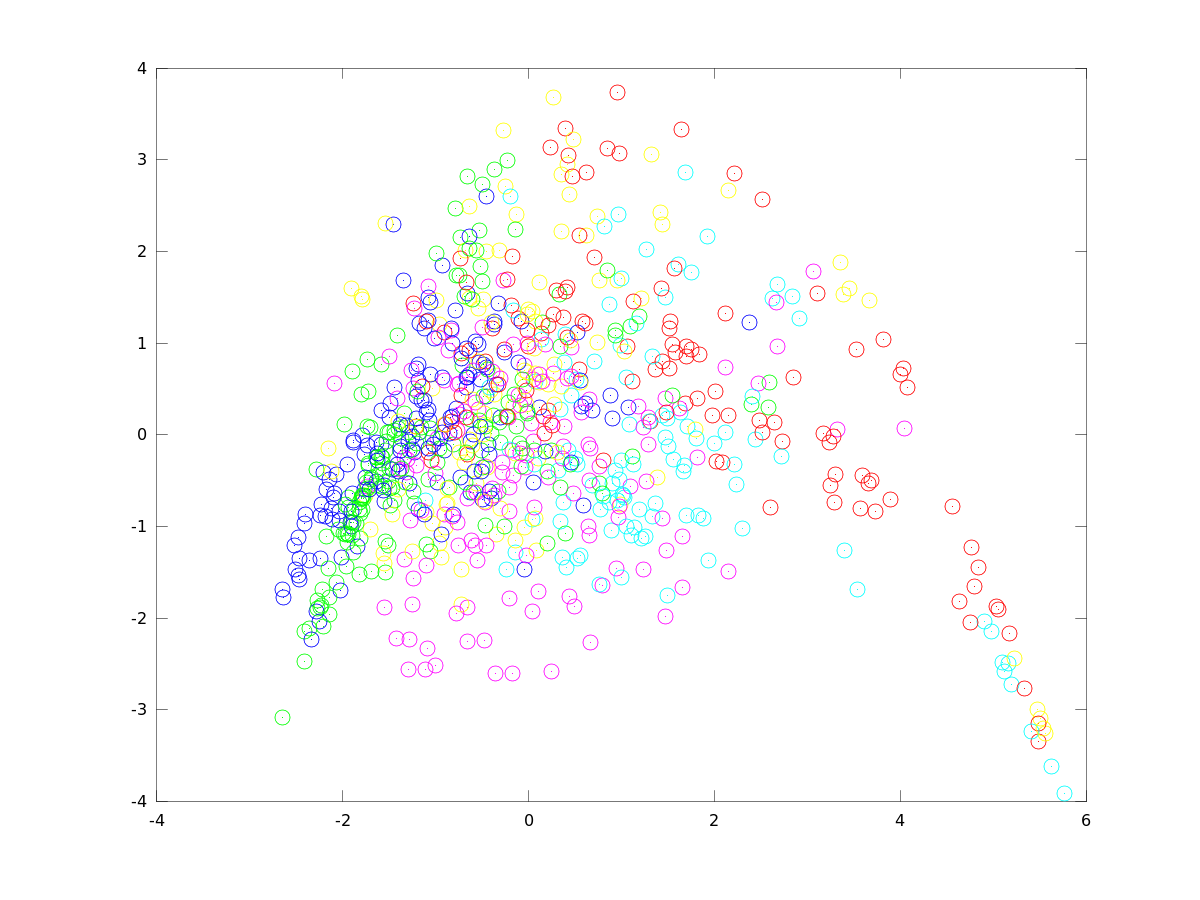
\includegraphics[width=6cm]{pca.png}
\label{fig:pca}
\end{figure}
\clearpage
\section{Conclusions}

This paper shows an approach to build a paper currency classifier, and shows the results for different
classification algorithms.

The data shows that the features are not linearly separable. The evidence that supports this argument is the
difference in the accuracy of the linear classifier against the multilayer perceptron. If the features were
linearly separable a higher accuracy would be expected on the linear classifier. The principal component
analysis algorithm \ref{fig:pca} also shows that data points of different classes are close in the same
regions of the space, but as the first 2 principal components only explain a 53.93\% of the variance, this
plot is not a strong argument to support this conclusion.

The final accuracy of the neural network was about 79\% while the accuracy of random system for the same problem would
be 16.6\%. To improve further this system, more data of a change in the feature vector could be a good idea. A
feature vector that would not discard the texture information could produce a better classifier.

\bibliographystyle{plain}
\bibliography{refs}

\end{document}
